\paragraph{Defining a function}

For functions there is a separation between the \emph{definition}, which describes what actions the function will perform, and the function \emph{call}, which signals that our function should be run. This also means that as we define a function, it will not automatically be run, allowing us to postpone running it until we need it. This, in turn, allows us to call a function multiple times in different parts of our programs. In this book, a function definition will look like this:

\begin{verbatim}
<type> <name of function>():
    <function body>
\end{verbatim}

For now, we will use \texttt{void} for the \texttt{<type>}. This word \texttt{void} signals that the function is intended to perform some action (later, we will see functions that calculate something). One example of a function that performs an action is a printing function:

\begin{verbatim}
void print_reassuring_message():
    print("I'm still here!")
\end{verbatim}

\paragraph{Calling a function}

Calling a function looks like this:

\begin{verbatim}
<name of function>()
\end{verbatim}

As you can see, the parentheses \texttt{()} are an important part of the function definition, as well as of the function call. Most programming languages use these to discern the use of functions from other elements of the program. Calling a function can be done from anywhere in the program as long as it has been \emph{defined} previously.

% TODO potential end note: the Ruby language makes () optional even for function calls, which means that the names of functions must be even more discerning than in other languages

\paragraph{Tracing} Function calls can be traced, but because the definition of a function and calls to functions are separate, we need a clear notation. Say we take the program below. The execution of the program starts at the first line that is not a function definition (in our case, the last line). On this line, the function \texttt{baz} is called. In the function \texttt{baz}, the function `bar` is called, which we can then \"jump\" to. The key is to strictly follow the top-down sequence of statements, unless there is a function call.

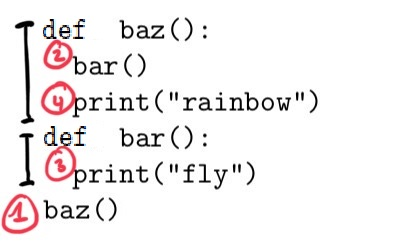
\includegraphics[width=.4\textwidth]{1-trace-calls.jpeg}

In our trace we put lines next to the two functions to have a clearly visible separation, and we number the lines in order of execution. We can see that \"fly\" is printed before \"rainbow\".
